\subsubsection{导数}

首先,我们来讨论一下函数的极限和连续性问题。设$w=f(z)$在$z_0$的邻域有定义,对于
$\epsilon > 0$,存在$\delta > 0$,使得$|z-z_0| < \epsilon$,有
\begin{equation}
    |f(z) - w_0| < \delta \textrm{,}
\end{equation}
称$z\to z_0$时$w_0$为$f(z)$的{\bf 极限},记为
\begin{equation}
    \lim_{z\to z_0} f(z) = w_0 \textrm{。}
\end{equation}
当$z$以任意方式趋近$z_0$时都有$ \lim_{z\to z_0} f(z) = w_0$,称$f(z)$在$z_0$点{\bf 连续}。
如果$f(z)$ 在$z_0=x_0 + \imath y_0$点连续,可以等价为
\begin{align}
    \lim_{\substack{x\to x_0\\y\to y_0}} \left(u(x,y), v(x,y)\right) = \left(u(x_0, y_0), v(x_0, y_0)\right) \textrm{。} 
\end{align}

复变函数的导数定义同实函数一样,定义为
\begin{align}
    \label{eq:derivative_def}
    f'(z) = \frac{df}{dz} 
    \equiv\lim_{\delta z \to 0} \frac{\delta w} {\delta z} 
    = \lim_{\delta z\to 0} \frac{f(z+\delta z) - f(z) } {(z+\delta z ) - z}
\end{align}
这里的前提条件是该极限与$\delta z \to 0$的方式无关。该极限为函数$f(z)$在$z$点的导数。通过该定义,实函数的求导公式对于复变函数同样试用,如
$(f+g)' = f' + g', (fg)' =f'g + fg'$等。与实变函数求导不同的是,复变函数导数存在条件是$\delta z$以任意方式趋于$0$,因而可导条件的要求比较严格。

\begin{figure}
    \centering
    \begin{tikzpicture}[scale=3]
    \draw[->] (-0.2,0) -- (1.2,0) node[right] {$\operatorname{Re}(z)$};
    \draw[->] (0,-0.2) -- (0,1.0) node[above] {$\operatorname{Im}(z)$};
    % \draw[dashed] (0.5,-1.5) -- (0.5,1.5);
    % \draw[dashed] (-1.5,0.5) -- (1.5,0.5);
    \draw[-latex] (1.0,0.3) -- (1.0,0.8) node[midway, right] {$\substack{\delta y\to 0\\\delta x=0}$};
    \draw[-latex] (0.3,0.8) -- (1.0,0.8) node[midway, above] {$\substack{\delta x\to 0\\\delta y=0}$};
    \filldraw [fill=none] (1,0.8) circle (0.02) node[above right] {$z_0$};
    \node at (0,0) [below left] {$O$};
\end{tikzpicture}
    \caption{逼近$z_0$的两种特殊方式。}
    \label{fig:limits}
\end{figure}
按照\ref{fig:limits}两种方式逼近$z_0$,我们可以得到
\begin{align}
    \lim _{\delta z \rightarrow 0} \frac{\delta f}{\delta z} &=\lim _{\delta x \rightarrow 0}\left(\frac{\delta u}{\delta x}+i \frac{\delta v}{\delta x}\right)=\frac{\partial u}{\partial x}+i \frac{\partial v}{\partial x},
\\
    \lim _{\delta z \rightarrow 0} \frac{\delta f}{\delta z} &=\lim _{\delta y \rightarrow 0}\left(-i \frac{\delta u}{\delta y}+\frac{\delta v}{\delta y}\right)=-i \frac{\partial u}{\partial y}+\frac{\partial v}{\partial y}
\end{align}
于是